% ========================================
%	Header einbinden
% ========================================

\documentclass[bibtotoc,titlepage]{scrartcl}

% Deutsche Spracheinstellungen
\usepackage[ngerman,german]{babel, varioref}
\usepackage[T1]{fontenc}
\usepackage[utf8]{inputenc}

%\usepackage{marvosym}

\usepackage{amsfonts}
\usepackage{amssymb}
\usepackage{amsmath}
\usepackage{amscd}
\usepackage{amstext}
\usepackage{float}
\usepackage{caption}
\usepackage{wrapfig}
\usepackage{setspace}
\usepackage{threeparttable}
\usepackage{footnote}

\usepackage{caption}
\usepackage{subcaption}

\newfloat{formel}{htbp}{for}
\floatname{formel}{Formel}


\usepackage{longtable}

%\usepackage{bibgerm}

\usepackage{footnpag}

\usepackage{ifthen}                 %%% package for conditionals in TeX
\usepackage{siunitx}
%Fr textumflossene Bilder und Tablellen
%\usepackage{floatflt} - veraltet

%Fr Testzwecke aktivieren, zeigt labels und refs im Text an.
%\usepackage{showkeys}

% Abstand zwischen zwei Abs�zen nach DIN (1,5 Zeilen)
% \setlength{\parskip}{1.5ex plus0.5ex minus0.5ex}

% Einrckung am Anfang eines neuen Absatzes nach DIN (keine)
%\setlength{\parindent}{0pt}

% R�der definieren
% \setlength{\oddsidemargin}{0.3cm}
% \setlength{\textwidth}{15.6cm}

% bessere Bildunterschriften
%\usepackage[center]{caption2}


% Probleml�ungen beim Umgang mit Gleitumgebungen
\usepackage{float}

% Nummeriert bis zur Strukturstufe 3 (also <section>, <subsection> und <subsubsection>)
%\setcounter{secnumdepth}{3}

% Fhrt das Inhaltsverzeichnis bis zur Strukturstufe 3
%\setcounter{tocdepth}{3}

\usepackage{exscale}

\newenvironment{dsm} {\begin{displaymath}} {\end{displaymath}}
\newenvironment{vars} {\begin{center}\scriptsize} {\normalsize \end{center}}


\newcommand {\en} {\varepsilon_0}               % Epsilon-Null aus der Elektrodynamik
\newcommand {\lap} {\; \mathbf{\Delta}}         % Laplace-Operator
\newcommand {\R} { \mathbb{R} }                 % Menge der reellen Zahlen
\newcommand {\e} { \ \mathbf{e} }               % Eulersche Zahl
\renewcommand {\i} { \mathbf{i} }               % komplexe Zahl i
\newcommand {\N} { \mathbb{N} }                 % Menge der nat. Zahlen
\newcommand {\C} { \mathbb{C} }                 % Menge der kompl. Zahlen
\newcommand {\Z} { \mathbb{Z} }                 % Menge der kompl. Zahlen
\newcommand {\limi}[1]{\lim_{#1 \rightarrow \infty}} % Limes unendlich
\newcommand {\sumi}[1]{\sum_{#1=0}^\infty}
\newcommand {\rot} {\; \mathrm{rot} \,}         % Rotation
\newcommand {\grad} {\; \mathrm{grad} \,}       % Gradient
\newcommand {\dive} {\; \mathrm{div} \,}        % Divergenz
\newcommand {\dx} {\; \mathrm{d} }              % Differential d
\newcommand {\cotanh} {\; \mathrm{cotanh} \,}   %Cotangenshyperbolicus
\newcommand {\asinh} {\; \mathrm{areasinh} \,}  %Area-Sinus-Hyp.
\newcommand {\acosh} {\; \mathrm{areacosh} \,}  %Area-Cosinus-H.
\newcommand {\atanh} {\; \mathrm{areatanh} \,}  %Area Tangens-H.
\newcommand {\acoth} {\; \mathrm{areacoth} \,}  % Area-cotangens
\newcommand {\Sp} {\; \mathrm{Sp} \,}
\newcommand {\mbe} {\stackrel{\text{!}}{=}}     %Must Be Equal
\newcommand{\qed} { \hfill $\square$\\}
\renewcommand{\i} {\imath}
\def\captionsngerman{\def\figurename{\textbf{Abb.}}}

%%%%%%%%%%%%%%%%%%%%%%%%%%%%%%%%%%%%%%%%%%%%%%%%%%%%%%%%%%%%%%%%%%%%%%%%%%%%
% SWITCH FOR PDFLATEX or LATEX
%%%%%%%%%%%%%%%%%%%%%%%%%%%%%%%%%%%%%%%%%%%%%%%%%%%%%%%%%%%%%%%%%%%%%%%%%%%%
%%%
\ifx\pdfoutput\undefined %%%%%%%%%%%%%%%%%%%%%%%%%%%%%%%%%%%%%%%%% LATEX %%%
%%%
\usepackage[dvips]{graphicx}       %%% graphics for dvips
\DeclareGraphicsExtensions{.eps,.ps}   %%% standard extension for included graphics
\usepackage[ps2pdf]{thumbpdf}      %%% thumbnails for ps2pdf
\usepackage[ps2pdf,                %%% hyper-references for ps2pdf
bookmarks=true,%                   %%% generate bookmarks ...
bookmarksnumbered=true,%           %%% ... with numbers
hypertexnames=false,%              %%% needed for correct links to figures !!!
breaklinks=true,%                  %%% breaks lines, but links are very small
linkbordercolor={0 0 1},%          %%% blue frames around links
pdfborder={0 0 112.0}]{hyperref}%  %%% border-width of frames
%                                      will be multiplied with 0.009 by ps2pdf
%
%\hypersetup{ pdfauthor   = {Hannes Franke; Julius Tilly},
%pdftitle    = {x}, pdfsubject  = {Protokoll FP}, pdfkeywords = {V301, Innenwiderstand, Leistungsanpassung},
%pdfcreator  = {LaTeX with hyperref package}, pdfproducer = {dvips
%+ ps2pdf} }
%%%
\else %%%%%%%%%%%%%%%%%%%%%%%%%%%%%%%%%%%%%%%%%%%%%%%%%%%%%%%%%% PDFLATEX %%%
%%%
\usepackage[pdftex]{graphicx}      %%% graphics for pdfLaTeX
\DeclareGraphicsExtensions{.pdf}   %%% standard extension for included graphics
\usepackage[pdftex]{thumbpdf}      %%% thumbnails for pdflatex
\usepackage[pdftex,                %%% hyper-references for pdflatex
bookmarks=true,%                   %%% generate bookmarks ...
bookmarksnumbered=true,%           %%% ... with numbers
hypertexnames=false,%              %%% needed for correct links to figures !!!
breaklinks=true,%                  %%% break links if exceeding a single line
linkbordercolor={0 0 1},
linktocpage]{hyperref} %%% blue frames around links
%                                  %%% pdfborder={0 0 1} is the default
% \hypersetup{
% pdftitle    = {V301 Innenwiderstand und Leistungsanpassung}, 
% pdfsubject  = {Protokoll AP}, 
% pdfkeywords = {V301, Innenwiderstand, Leistungsanpassung},
% pdfsubject  = {Protokoll AP},
% pdfkeywords = {V301, Innenwiderstand, Leistungsanpassung}}
%                                  %%% pdfcreator, pdfproducer,
%                                      and CreationDate are automatically set
%                                      by pdflatex !!!
\pdfadjustspacing=1                %%% force LaTeX-like character spacing
\usepackage{epstopdf}
%
\fi %%%%%%%%%%%%%%%%%%%%%%%%%%%%%%%%%%%%%%%%%%%%%%%%%%% END OF CONDITION %%%
%%%%%%%%%%%%%%%%%%%%%%%%%%%%%%%%%%%%%%%%%%%%%%%%%%%%%%%%%%%%%%%%%%%%%%%%%%%%
% seitliche Tabellen und Abbildungen
%\usepackage{rotating}
\usepackage{ae}
\usepackage{
  array,
  booktabs,
  dcolumn
}
\makeatletter 
  \renewenvironment{figure}[1][] {% 
    \ifthenelse{\equal{#1}{}}{% 
      \@float{figure} 
    }{% 
      \@float{figure}[#1]% 
    }% 
    \centering 
  }{% 
    \end@float 
  } 
  \makeatother 


  \makeatletter 
  \renewenvironment{table}[1][] {% 
    \ifthenelse{\equal{#1}{}}{% 
      \@float{table} 
    }{% 
      \@float{table}[#1]% 
    }% 
    \centering 
  }{% 
    \end@float 
  } 
  \makeatother 
%\usepackage{listings}
%\lstloadlanguages{[Visual]Basic}
%\allowdisplaybreaks[1]
%\usepackage{hycap}
%\usepackage{fancyunits}
\usepackage{xfrac}
\sisetup{output-decimal-marker = {,}}

% ========================================
%	Angaben für das Titelblatt
% ========================================

\title{V01 - Lebensdauer der Myonen\\				% Titel des Versuchs 
\large TU Dortmund, Fakultät Physik\\ 
\normalsize Fortgeschrittenen-Praktikum}

\author{Jan Latarius\\			% Name Praktikumspartner A
{\small \href{jan.latarius@tu-dortmund.de}{jan.latarius@tu-dortmund.de}}	% Erzeugt interaktiven einen Link
\and						% um einen weiteren Author hinzuzfügen
Dimitrios Skodras\\					% Name Praktikumspartner B
{\small \href{dimitrios.skodras@tu-dortmund.de}{dimitrios.skodras@tu-dortmund.de}}		% Erzeugt interaktiven einen Link
}
\date{19.12.2016}				% Das Datum der Versuchsdurchführung

% ========================================
%	Das Dokument beginnt
% ========================================

\begin{document}

% ========================================
%	Titelblatt erzeugen
% ========================================

\maketitle					% Jetzt wird die Titelseite erzeugt
\thispagestyle{empty} 				% Weder Kopfzeile noch Fußzeile

% ========================================
%	Der Vorspann
% ========================================

%\newpage					% Wenn Verzeichnisse auf einer neuen Seite beginnen sollen
%\pagestyle{empty}				% Weder Kopf- noch Fußzeile für Verzeichnisse

\tableofcontents

%\newpage					% eine neue Seite
%\thispagestyle{empty}				% Weder Kopf- noch Fußzeile für Verzeichnisse
%\listoffigures					% Abbildungsverzeichnis

%\newpage					% eine neue Seite
%\thispagestyle{empty}				% Weder Kopf- noch Fußzeile für Verzeichnisse
%\listoftables					% Tabellenverzeichnis
\newpage					% eine neue Seite


% ========================================
%	Kapitel
% ========================================

%\section{Einleitung}				% Bei Bedarf

\section{Ziel}
%Ziel dieses Versuches ist es, die mittlere Lebensdauer kosmischer Myonen, d.h. die  charakteristische Zeit des statistischen Zerfallsprozess, zu bestimmen. Dafür wird eine elektronische Messapparatur aufgebaut und kalibriert. 
Mit diesem Versuch soll die mittlere Lebensdauer von kosmischen Myonen bestimmt werden. Im Laufe des Versuchs wird zum einen der Aufbau getestet und kalibriert, anschließend wird über mehrere Tage die Anzahl der Zerfälle gemessen.

\section{Theorie}
\subsection{Einleitung}
Im Standardmodell wird zwischen Fermionen und Bosonen unterschieden: Erstere haben einen halbzahligen, letztere einen ganzzahligen Spin. Fermionen werden weiterhin in Quarks und Leptonen unterteilt, je nachdem ob sie stark wechselwirken oder nicht. 

Der bekannteste Vertreter der Leptonen ist das Elektron. Neben diesem Beispiel aus der 1. Generation der Leptonen gibt es noch schwerere Vertreter wie das Myon und das Tauon aus der 2. und 3. Generation. Im Gegensatz zum Elektron sind diese nicht stabil und zerfallen nach einer entsprechenden Zerfallsstatistik. Dar\"uber hinaus existieren f\"ur jede Generation auch noch Neutrinos und die Antiteilchen zu allen genannten Teilchen.

Hier sind vor allem die Myonen interessant, deren mittlere Zerfallsdauer in diesem Experiment bestimmt werden soll.

\subsection{Zerfall vom Myon}
Das Myon ist ca. 206-mal schwerer als das Elektron, es besitzt genauso wie sein leichterer Verwandter einen Spin $\frac{1}{2}$. Auf der Erde kommen Myonen vor allem in der oberen Atmosph\"are vor, wo sie durch die Interaktion von Sonnenwind mit Luftmolekülen aus dem Zerfall von Pionen entstehen:

\begin{align*}
	\pi^+ \rightarrow \mu^+ + \nu_\mu\\	
	\pi^- \rightarrow \mu^- + \overline{\nu}_\mu.
\end{align*}

Diese kosmischen Myonen besitzen eine hohe kinetische Energie, sodass sie teilweise erst am Boden zerfallen, wo sie f\"ur uns messbar sind:

\begin{align*}
	\mu^+ \rightarrow e^+ + \nu_e + \bar{\nu}_\mu\\
	\mu^- \rightarrow e^- + \bar{\nu}_e + \nu_\mu
\end{align*}

Der Teilchenzerfall ist ein statistischer Prozess, der durch die mittlere Lebensdauer $\tau$ charakterisiert wird. Die Wahrscheinlichkeit, dass ein Teilchen zerf\"allt, kann differentiell geschrieben werden als

\begin{align}
	\text{d}W = \lambda \text{d}t.
\end{align}

Bei einer hinreichend gro{\ss}en Teilchenzahl $N$ und aufgrund der statistischen Unabhängigkeit der Ereignisse ist die mittlere \"Anderung der Teilchenzahl gegeben durch

\begin{align*}
	\text{d}N = - N \text{d}W = - \lambda \text{d}t,
\end{align*}

wenn dies integriert wird, folgt daraus das Zerfallsgesetz

\begin{align}
	N(t) = N_0 e^{-\lambda t}.
	\label{eq:zerfallsgesetz}
\end{align}

Daraus l\"asst sich die \"Anderung der Teilchenzahl im Zeitraum [$t$,$t+$d$t$] bestimmen:

\begin{align}
	\frac{\text{d}N(t)}{N_0} = \frac{N(t)-N(t+\text{d}t)}{N_0} = \lambda e^{-\lambda t}\text{d}t,
	\label{eq:lebensdauer}
\end{align}

dies entspricht der Verteilung der Lebensdauern der zerfallenden Teilchen. Wird nun die mittlere Lebensdauer $\tau$ als der Erwartungswert dieser Verteilung bestimmt, so ist

\begin{align}
	\tau = \int_{0}^{\infty} \lambda t e^{-\lambda t}\text{d}t = \frac{1}{\lambda}.
\end{align}

\subsection{Absch\"atzung der Lebensdauer}
Da keine unendlich langen Messzeiten zur Verf\"ugung stehen, muss die mittlere Lebensdauer mithilfe von endlichen Messungen abgesch\"atzt werden.

Dazu werden gemessene Lebensdauern gemittelt:

\begin{align}
	\tau = \langle t \rangle = \frac{1}{n} \sum_{i=1}^{n} t_i,
\end{align}

wobei der Fehler dieser Mittelung gegeben ist durch

\begin{align}
	s(\tau) = \frac{1}{\sqrt{n(n-1)}} \sum_{i=1}^{n} (\langle t \rangle - t_i)^2 .
\end{align}

M\"ogliche systematische Fehler dieser Mittelung z.B. durch Abschneiden zu gro{\ss}er und zu kleiner Messwerte aufgrund des Messaufbaus werden durch einen exponentiellen Fit der empirischen Verteilungsfunktion ausgeglichen.

\section{Aufbau}
\subsection{Messapparatur}
Kosmische Myonen entstehen in der oberen Atmosph\"are aus dem Zerfall von Pionen. Sie besitzen dann meist eine kinetische Energie im GeV-Bereich. Auf der Erdoberfl\"ache wird nun mithilfe einer Szintillationskammer die Energieabgabe der Myonen, die sich durch die Kammer bewegen, durch Bremsstrahlung bzw. einen Lichtblitz messbar. 

Die Myonen werden sowohl durch die Atmosph\"are als auch das beinhaltende Geb\"aude meist stark abgebremst. Deswegen kann es sein, dass einfallende Myonen in der Sintillatorkammer bis zum Stillstand abgebremst werden, sodass dort ihre eigentliche Lebensdauer bestimmt werden kann. Dies f\"uhrt zu einem weiteren Lichtblitz, der aufgrund der entstehenden hochenergetischen Elektronen und Positronen als Zerfallsprodukte entsteht. Der zeitliche Abstand dieser Signale entspricht der Lebensdauer eines Myons.

\begin{figure}[t]
	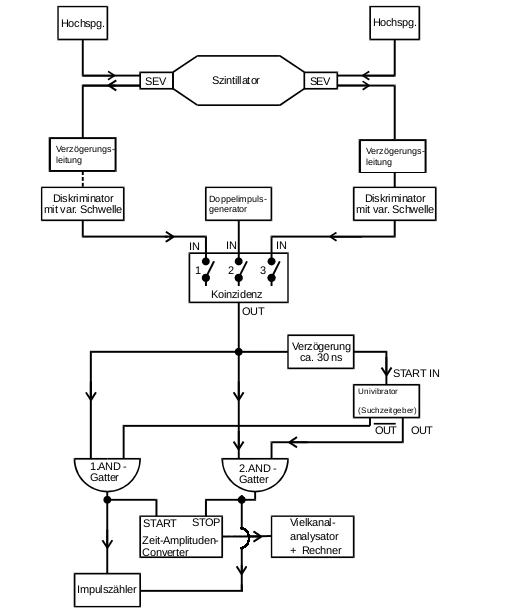
\includegraphics[width=0.7\textwidth]{../pics/blockAdaptiert.png}
	\caption{Schaltplan der verwandten, adaptierten Messaparatur \cite{Anl}}
	\label{pic:setup}
\end{figure}

In Abb. \ref{pic:setup} ist der benutzte Aufbau zu sehen. Kernst\"uck ist die Szintillatorkammer mit einem Volumen von 50\,l. In diesem Beh\"altnis ist ein organischer Szintillator mit kleiner Totzeit gegen\"uber der Lebensdauer von Myonen. Daran an gegen\"uberliegenden Seiten angeschlossen sind zwei Sekund\"arelektronenvervielfacher (SEV), die optisch mit der Kammer verbunden sind. Durch ihre Photokathode werden auftretende Signale registriert und verst\"arkt. Diese dienen nach Umwandlung als Start- und Endimpulse f\"ur das Z\"ahlwerk.

Da die SEVs nicht komplettt symmetrisch angeschlossen sind, wird durch eine Verz\"ogerungsleitung der zeitliche Unterschied austariert. Weiterhin sorgt eine Diskriminatorschwelle daf\"ur, dass nur Impulse oberhalb einer Schwelle wahrgenommen werden, damit m\"oglichst viel der Untergrundstrahlung bereits hier ausgeblendet wird, und wandelt die unterschiedlich starken und breiten Pulse in NIM-Pulse um. Eine Koinzidenzschaltung sorgt daf\"ur, dass die beiden Impulse aus den SEVs zeitlich als einer registriert werden. 

Diese zeitlichen Abst\"ande werden durch einen time amplitude converter (TAC) in eine entsprechende Spannung umgewandelt, die wiederum von einem Vielkanalanalysator im Computer in 512 Kan\"ale sortiert wird. Dies dient als Ausgangspunkt f\"ur die Auswertung zur Bestimmung der Lebensdauer von Myonen.

Zur Messung der Lebensdauer sollen die Signale beim Eintritt und beim Zerfall als Start- und Stopsignal registriert werden. Da nicht alle Myonen innerhalb der Szintillatorkammer komplett abgebremst werden, werden h\"aufig nur ein Start- und kein Endimpulse registriert. Dies wird in der Schaltung ber\"ucksichtigt: Dazu wird eine monostabile Kippschaltung oder Univibrator hinter einer Verz\"ogerungsleitung eingesetzt. Sie bewirkt, dass am AND-Gatter f\"ur Startimpulse Eingang 1 ein HIGH-Signal einl\"auft (HIGH und LOW entstammen dem NIM-Standard als bin\"are Logik f\"ur elektronische Schaltungen). Sobald der Startpuls vorbei ist, schlie{\ss}t der Univibrator das Start-AND wieder und dies wird als Eingangsimpuls beim TAC registriert. Entsprechend wird beim Endpuls das End-AND ge\"offnet und wieder geschlossen. Kommt es zu keinem Endpuls, so setzt der Univibrator die Schaltung wieder zurück.

Hier wird eine weitere Fehlerquelle ersichtlich: Im Fall von zwei Myonen, die kurz nacheinander die Kammer durchqueren, kann dies als ein zerfallenes Myon interpretiert werden. Diese seltenen Ereignisse werden als Untergrund $U$ ber\"ucksichtigt. Als seltene Ereignisse werden sie durch die Poisson-Verteilung beschrieben, weiterhin kann mit der mittleren Z\"ahlrate und der Messdauer dieser Untergrund abgesch\"atzt werden.

Eine weitere Fehlerquelle ist das thermische Rauschen der SEVs. Dabei kommt es zur thermischen Emission von Elektronen, die mit verst\"arkt werden und somit auch zu den Fehlerimpulsen beitragen. Diese Impulse sind aber schw\"acher als die der Myonen, sodass sie durch zwischengeschaltete Diskriminatoren unterdr\"uckt werden.

\subsection{Kalibration}
Zuerst wird der zeitliche Unterschied zwischen den SEVs mithilfe eines Doppelimpulsgenerators bestimmt. Dieser Unterschied wird daraufhin durch Einf\"ugen einer Verz\"ogerungsleitung ausgeglichen. Ziel ist die Maximierung der Z\"ahlrate nach der Koinzidenzschaltung.

Weiterhin werden die Schwellwerte der Diskriminatoren eingeregelt. Au{\ss}erdem wird f\"ur den Univibrator passende Suchdauer gew\"ahlt.

Abschlie{\ss}end wird die Zeitkonstante des Vielkanalanalysators so gew\"ahlt, dass f\"ur die angestrebte gesamte Messdauer eine angemessene zeitliche Aufl\"osung gew\"ahrleistet ist.



%\section{Durchführung}
\label{sec:exec}

\section{Auswertung}
\subsection{Verzögerungsleitung}
Wie in Abbildung \ref{pic:setup} dargestellt und in Abschnitt \ref{sec:exec} beschrieben, soll gewährleistet werden, dass die Signale der SEVs 
gleichzeitig zur Koinzidenzapparatur gelangen. Die Verzögerung, erreicht mit hinzukommender Kabellänge sowie ihr Einfluss auf die Signalrate
sind in Tabelle \ref{tab:koinz} aufgeführt und in \ref{pic:koinz} dargestellt. 
\begin{figure}[t]
 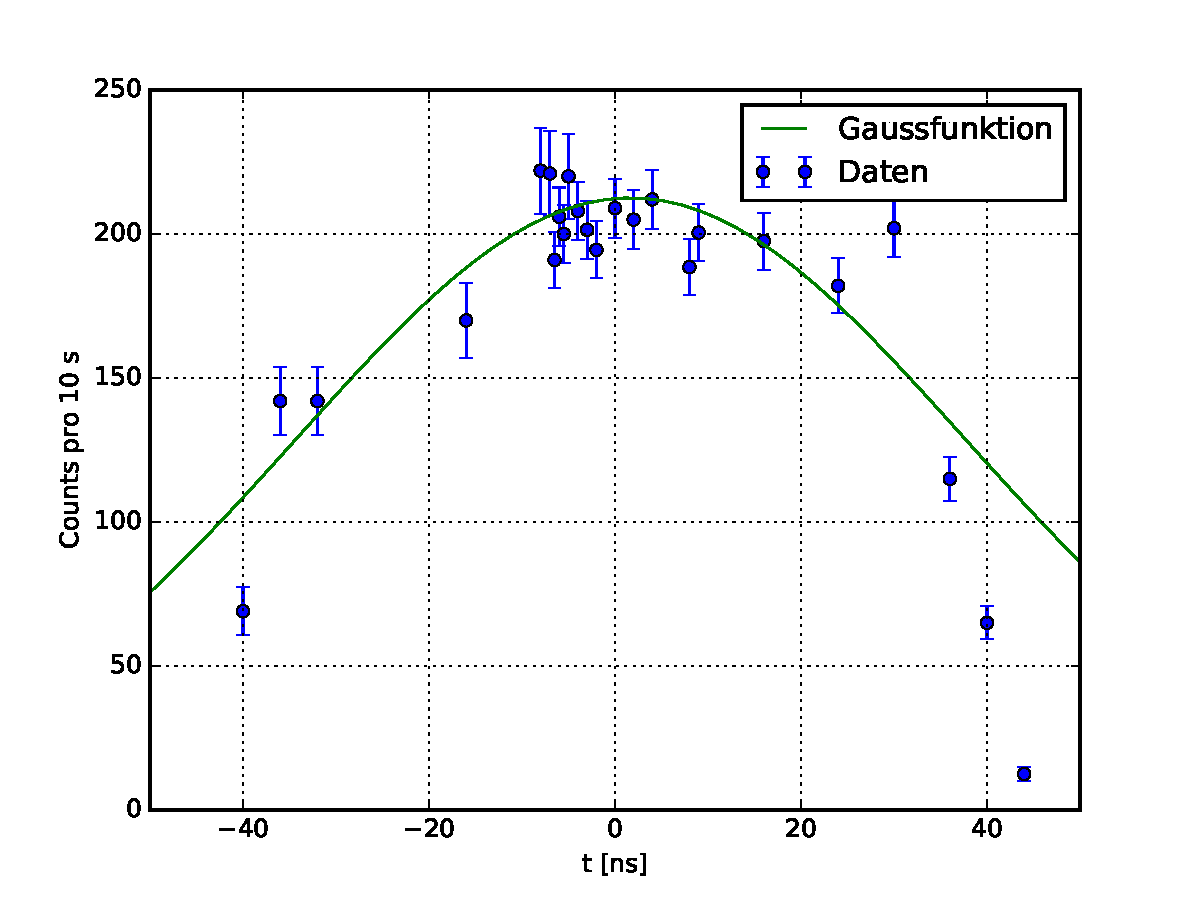
\includegraphics[width=0.7\textwidth]{../pics/koinzidenz.pdf}
 \caption{Zählraten entsprechender Verzögerungen. Die benutzte Verzögerungsleitung sowie der Zusammenhang zur Pulsbreite sollen mit einer 
 Gaussfunktion näher betrachtet werden.}
 \label{pic:koinz}
\end{figure}
Man erkennt eine relativ geringe Einflussnahme der Verzögerung entsprechend des breiten Plateaus,
weshalb angenommen wird, dass der tatsächlichen Wahl eine gewisse Freiheit beiwohnt. 
Während der Versuchsdurchführung ist die Verzögungsleitung auf \SI{-3}{\nano\second} angestellt worden, da die abfallenden Flanken an den 
Rändern der Messreihe darum zentriert sind. 
\begin{table}[b]
\input{../auswertung/koinzidenz.dat}
\caption{Verzögerungsleitung zur Synchronisierung der SEVs. Negative $t$ entsprechen einer Verzögerung des linken SEVs. In der dritten Spalte 
sind die Zählraten auf 10\,s Messzeit aufgeführt.}
\label{tab:koinz}
\end{table}
Entsprechend des Myonenstroms \cite{pdg} werden die Diskriminatoren einer Rate von 20-30\,\si{\per\second} \cite{Anl} entsprechend eingestellt. Die 
Pulsbreite wird am Oszillator zu \SI{11,5}{\nano\second} abgelesen. Der Fit der Gaussfunktion an die Messreihe 
\begin{align}
 f(x) = A\exp\left[-\left(\frac{x-\mu}{\sigma}\right)^2\right]
\end{align}
liefert
\begin{align}
 A &= 212(5)\\
 \mu &=  \SI{1.7(13)}{\nano\second}\\
 \sigma &= \SI{51(3)}{\nano\second}.
\end{align}
Die gewählte Verzögerung liegt im angegebenen Bereich des Mittelwerts $\mu$. Wenn die Pulse mit ihrer vorderen bzw. hinteren Flanke an der 
Koinzidenz ankommen, werden die Ereignisse als Counts gezählt. Entsprechend sollte man eine Halbwertsbreite von der etwa doppelten Pulsbreite,
also \SI{13}{\nano\second}. Für Normalverteilungen ist die Halbwertsbreite $\sim 2,4\,\sigma \approx \SI{120}{\nano\second}$ \cite{standard}, also etwa 9-mal
so groß. Die Toleranz der Koinzidenz $\Delta t_K \gtrsim \SI{4}{\nano\second}$ reicht zur Erklärung hierzu jedenfalls nicht aus. 
Ein fehlerhaftes Ablesen der Pulsbreite könnte eine Ursache für diese Diskrepanz sein. 


\subsection{Kalibrierung der Zeitachse}
Die Zeitdifferenz $\Delta t$ zwischen zwei vom Doppelimpulsgenerator Signalen wird vom TAC in eine Spannung umgewandelt, die vom Vielkanalanalysator 
ausgelesen wird. Diese Differenz wird in \SI{1}{\nano\second}-Schritten von \SI{1}{\nano\second} bis \SI{9}{\nano\second} variiert und geprüft,
welchem Kanal sie zugeordnet wird \footnote[1]{Aufgrund eines mutmaßlichen, technischen Fehlers des TACs sind die zur weiteren Auswertung benötigten
Daten vom Versuchsbetreuer \href{robert.theinert@tu-dortmund.de}{Robert Theinert} gestellt worden.}. Der sich abzeichnende lineare Zusammenhang
\begin{align}
 f(x) = ax + b
\end{align}
ist in Abbildung \ref{pic:linfit} 
\begin{figure}[t]
 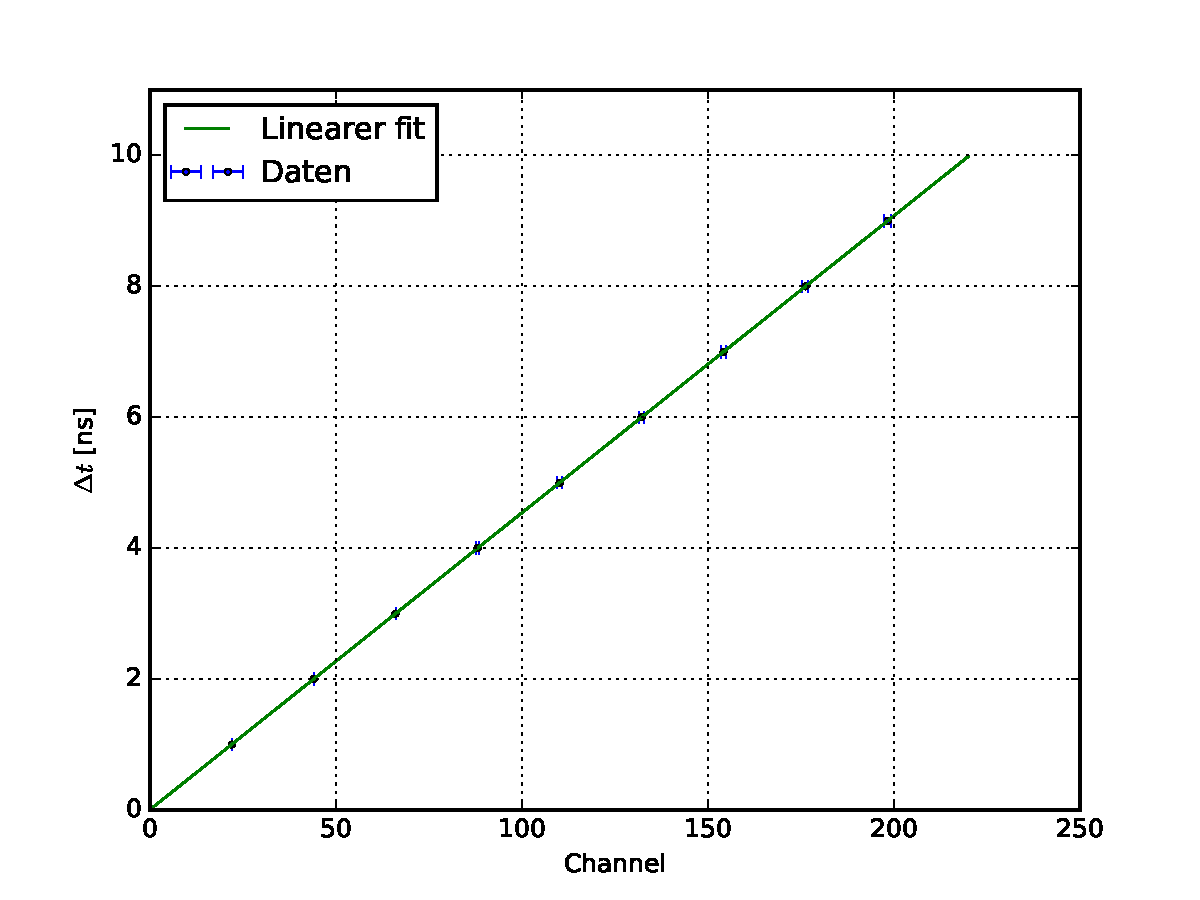
\includegraphics[width=0.7\textwidth]{../pics/linFit}
 \caption{Linearer Zusammenhang zwischen der Spannungsamplitude entsprechenden Zeitdifferenz $\Delta t$ und dem jeweiligen Kanal des 
 Vielkanalanalysators.}
 \label{pic:linfit}
\end{figure}
dargestellt und seine Fitparameter, bestimmt durch \texttt{Python3.6} mithilfe des Moduls \texttt{scipy.optimize}, ergeben sich zu
\begin{align}
 a&= \SI{4,54(1)e-2}{\nano\second\per Kanal}\\
 b&= \SI{5,50(1)e-3}{\nano\second}.
 \label{eq:kalibparams}
\end{align}
Die Berechnung bezieht nur die ersten 200 Kanäle mit ein, jedoch sind 512 vorhanden, weshalb der lineare Zusammenhang aufgrund des kleinen Fehlers
fortgeführt wird.
Es kommt beim Auslesen teilweise zu einer Zuordnung auf mehrere, direkt nebeneinanderliegende Kanäle sodass ein gewichtetes Mittel verwandt wird.
Der dadurch entstehende Fehler hat einen verschwindenden Einfluss auf die Fitparameter. Weiterhin gibt es Fälle, in denen kleine Fluktuationen
von einem Count in einem beliebigen Kanal auftauchen. Diese werden nicht berücksichtigt.
\subsection{Bestimmung der Untergrundrate}
Während einer Messzeit von $t_\text{mess}=\SI{1449146}{\second}$ werden $N_\text{start}=\SI{32201706}{}$ Anfangsimpulse gezählt, was einer Rate von 
\begin{align}
 \bar N = \frac{N_\text{start}}{t_\text{mess}} = \SI{22,22(1)}{\per\second}
\end{align}
entspricht. Dies liegt im erwarteten Bereich, was darauf schließen lässt, dass die meisten Untergrundsignale von den Diskriminatoren herausgefiltert
worden sind. Während der Suchzeit $t_S=\SI{22}{\micro\second}$ kann ein zweites Myon in den Tank eintreten. Das daherrührende Untergrundsignal kann
mit der Poisson-Verteilung abgeschätzt werden. Dass genau ein weiteres Myon eintritt, entspricht einer Wahrscheinlichkeit von
\begin{align}
 P(n=1) = \bar N t_S \e^{-\bar N t_S} = \SI{4,886(1)e-4}{},
\end{align}
sodass also 
\begin{align}
 N_b = P(n=1)N_\text{start} = \SI{15735(6)}{}.
\end{align}
Hintergrundsignale sich gleichmäßig auf die Kanal mit $\Delta t < t_S$ verteilen. Aus \eqref{eq:kalibparams} ergibt sich die Anzahl beteiligter 
Kanäle zu
\begin{align}
 \text{Kanal}_\text{max} = t_S\frac{1}{a} - \frac{b}{a}  = 484,84(1),
\end{align}
womit die Untergrundsignale mit
\begin{align}
 U_\text{th} = \frac{N_b}{\text{Kanal}_\text{max}} = \SI{32,45(1)}{1\per Kanal}
 \label{eq:backgrTh}
\end{align}
zu erwarten sind.

\subsection{Bestimmung der Lebensdauer von Myonen}
Mit dem Zusammenhang der Zeitdifferenz des Start- und Stoppimpulses und den Kanälen lässt sich die Messung\footnote[2]{Die Daten hierfür sind ebenfalls
vom Versuchsbetreuer gestellt worden.} in Abbildung \ref{pic:lebensdauer} darstellen.
\begin{figure}[t]
 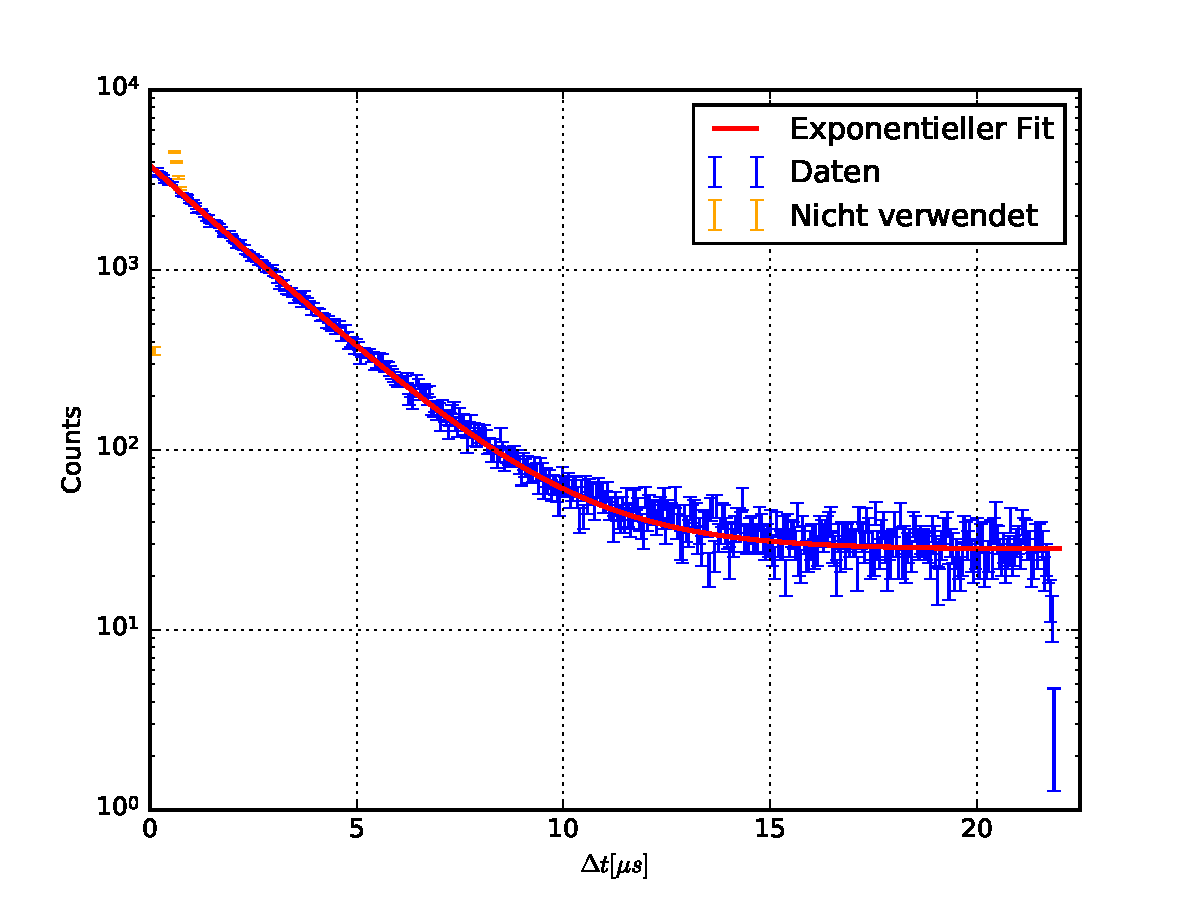
\includegraphics[width=0.8\textwidth]{../pics/lebensdauer_fit}
 \caption{Gemessene Start-Stoppimpulse bei entsprechenden Zerfallsdauern. Der Fit schließt die ersten drei Kanäle, die Kanäle 14, 15, 16 und 17, sowie
 alle Kanäle deren Pendant der Zeitdifferenz größer als $t_S$ ist.}
 \label{pic:lebensdauer}
\end{figure}
Einige Kanäle sind bei der Auswertung nicht miteinbezogen. Die ersten beiden Kanäle entsprechen einer zu kurzen Zerfallszeit,
die die Apparatur offenbar nicht auflösen kann. Die Kanäle 14-17 weisen Ausreißer auf, für die keine vernünftige Begründung gefunden worden ist.
Kanäle größer $t_S$ sind leer, sodass diese ebenfalls vernachlässigt werden.
Die Exponentialverteilung
\begin{align}
 f(\Delta t) = N_0 \e^{-{\sfrac{1}{\tau}}\,\Delta t} + U_\text{fit}
\end{align}
wird zum Kurvenverlauf angenommen. Der Fit wird unter der Gewichtung der inversen Standardabweichung erstellt,
der für die mittlere Lebensdauer
\begin{align}
 \tau = \SI{2,106(7)}{\micro\second}
 \label{eq:tau}
\end{align}
und den Untergrund
\begin{align}
 U_\text{fit} = \SI{28,16(140)}{1\per Kanal}
 \label{eq:backgrExp}
\end{align}
angibt. Weiterhin ist
\begin{align}
 N_0 = 378(9).
\end{align}

\section{Diskussion}
Nach der Messung stehen \SI{32201706}{} Startsignale \SI{201862}{} Stoppsignalen gegenüber, sodass \SI{0,63}{\%} der einfallenden Myonen tatsächlich
im Detektor zerfallen. Dies rechtfertigt eine lange Messdauer von 16 Tagen, um eine aussagekräftige Statistik zu ermöglichen. \\
\noindent Die erwartete \eqref{eq:backgrTh} und die gemessene \eqref{eq:backgrExp} Untergrundrate haben eine Abweichung von \SI{14}{\%} bzw.
3,06\,$\sigma$ zueinander,
wobei die gemessene geringer ist. Dies kann daher rühren, dass die Ausreißer im Datenset nicht mit in den Fit einbezogen wurden, jedoch den zu
erwartenden Untergrund beeinflussen. \\
\noindent Während $N_\text{stopp} = \SI{201862}{}$ sind in den Kanälen $N_\text{hist} = \SI{183911}{}$ gezählt. Die fehlenden Einträge sind insbesondere
in den ersten drei Bins feststellbar, die verglichen mit den anderen (fast) leer sind, aber erwartungsgemäß sehr voll sein müssten. Es scheint,
als würden der TAC oder der Vielkanalanalysator die entsprechend kurzzeitigen Signale nicht erfassen kann. Die verbliebenen, fehlenden Einträge
können an einer zu geringen Sensitivität zum Impulszähler liegen.\\
\noindent Ziel des Versuchs war es, die Lebensdauer von Myonen zu bestimmen. Diese ließ sich bestimmen zu $\tau = \SI{2,106(7)}{\micro\second}$,
was \SI{4,1}{\%} bzw. 13,0\,$\sigma$ unter dem Referenzwert \cite{pdg} von \SI{2,197}{\micro\second} liegt. Diese Differenz lässt sich damit erklären, dass die mittlere
Lebensdauer von Teilchen im Vakuum von der im Medium sich unterscheiden und die Wechselwirkung, wie das Muoncapturing \cite{mCapture}
zu einem schnelleren Zerfall führen. Ob weitere Effekte oder systematische Fehler noch miteinbezogen werden müssen, lässt sich nicht ausschließen.
Weiterhin wird der Fehler durch die nicht miteinbezogenen Kanäle verkleinert, sodass der durchaus signifikante
Unterschied vergrößert ist.


%\parskip 340pt
%\Large{Literatur}\\\\
\newpage
 \begin{thebibliography}{WissOnl}
 	\bibitem{Anl} TU Dortmund Anleitung für Versuch Nr.01 \url{http://129.217.224.2/HOMEPAGE/Anleitung_FPBSc.html}
 	\bibitem{pdg} C. Patrignani et al. (Particle Data Group), Chin. Phys. C, 40, 100001 (2016).
   	\bibitem{mCapture}   T.~Gorringe and H.~W.~Fearing,
    \textit{Induced pseudoscalar coupling of the proton weak interaction},
    Rev.\ Mod.\ Phys.\  {\bf 76}, 31 (2004)
    doi:10.1103/RevModPhys.76.31
    [nucl-th/0206039].
    \bibitem{standard} Weisstein, Eric W. "Gaussian Function." From MathWorld--A Wolfram Web Resource. \url{http://mathworld.wolfram.com/GaussianFunction.html }
	\end{thebibliography}

% ========================================
%	Literaturverzeichnis
% ========================================

%\bibliographystyle{plainnat}			% Bibliographie-Style auswählen
%\bibliography{BIBDATEI}			% Literaturverzeichnis

% ========================================
%	Das Dokument endent
% ========================================

\end{document}
